\chapter{Evaluation\label{cha:chapter7}}

In this chapter the implementation of the Rollup System is evaluated.
\todo[inline]{Write something}


% Put some screenshots in this section! Map the requirements with your proposed solution. Compare it with related work. Why is your solution better than a concurrent approach from another organization?

\section{Test Environment\label{sec:testenvir}}

ISE's department offers a server for executing the Rollup System. The server is equipped with an Intel Xeon CPU E3-1270 v6 @ 3.80GHz, 64GB DDR4 RAM, 32 GB of SWAP memory and 250GB of SSD storage. The server runs Gentoo release 2.7 Linux distribution with kernel version 5.10.52. When elsewhere specified it has been used a Google Cloud Platform virtual machine with 12 vCPU Intel Haswell, 256GB of RAM and 300 GB of SSD. This machine runs Debian 11.

The blockchain used for the Rollup System is the Tezos blockchain running on the Ghostnet testnet, with Nairobi Protocol. The RPC node used is \url{https://ghostnet.ecadinfra.com/}.


\section{Benchmarks\label{sec:benchmarks}}

\subsection{Hash Function\label{subsec:6_hashfunc}}

The hash function decision has been a key point to make the system more responsive and efficient, as the generation of the Merkle Trees and the merging process of balances and nonces rely on it. The initial programs were using sha256, but it was too RAM demanding and it was not possible to compile programs with more than 8 users. The implementation of the programs has been changed to use sha3, which revealed to be faster: ZoKrates sha256, in fact, adds a layer of complexity to the computation because it adds 256 bits of padding to the input, and involves more constraints in the computation. The sha3 adoption allowed performance increase without changing the rest of the program, as the inputs size and outputs were the same as sha256.
Finally the hash function has then been changed to Poseidon, which is very zk-SNARK friendly, allowing the compilation of programs up to 2048 users but it required some changes in the programs. Figure \ref{fig:7_sheets-benchmarks_hash.png} shows the RAM requirements for each hash function during the compile phase\footnote{A GCP machine has been used for RAM usage above 60 GB} compared to the amount of users and transactions.

\begin{figure}
	\centering
	\begin{minipage}{.48\textwidth}
		\centering
		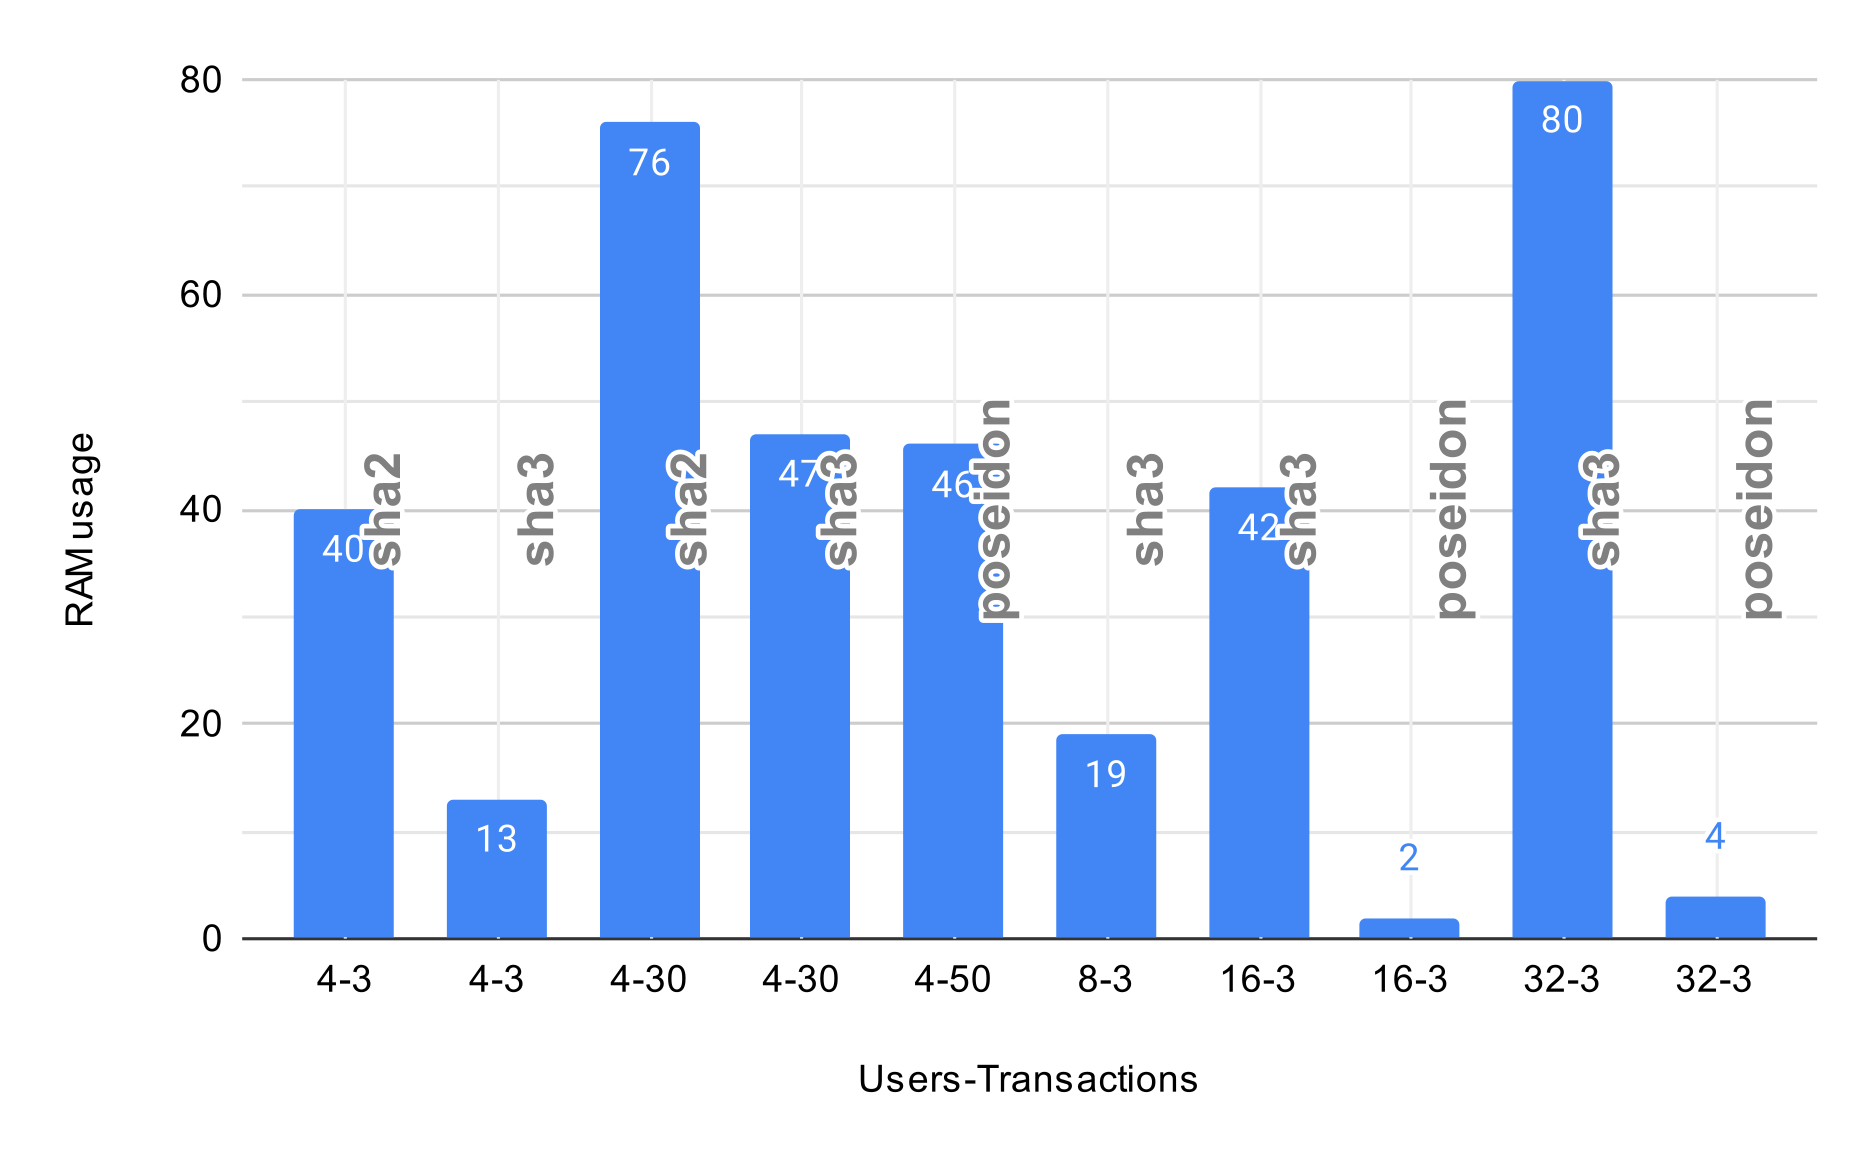
\includegraphics[width=\linewidth]{6_sheets-benchmarks_hash.png}
		\caption[RAM Usage hash]{RAM for each hash type. \newline x:users-transactions y:RAM}
		\label{fig:7_sheets-benchmarks_hash.png}
	\end{minipage}
	\begin{minipage}{.48\textwidth}
		\centering
		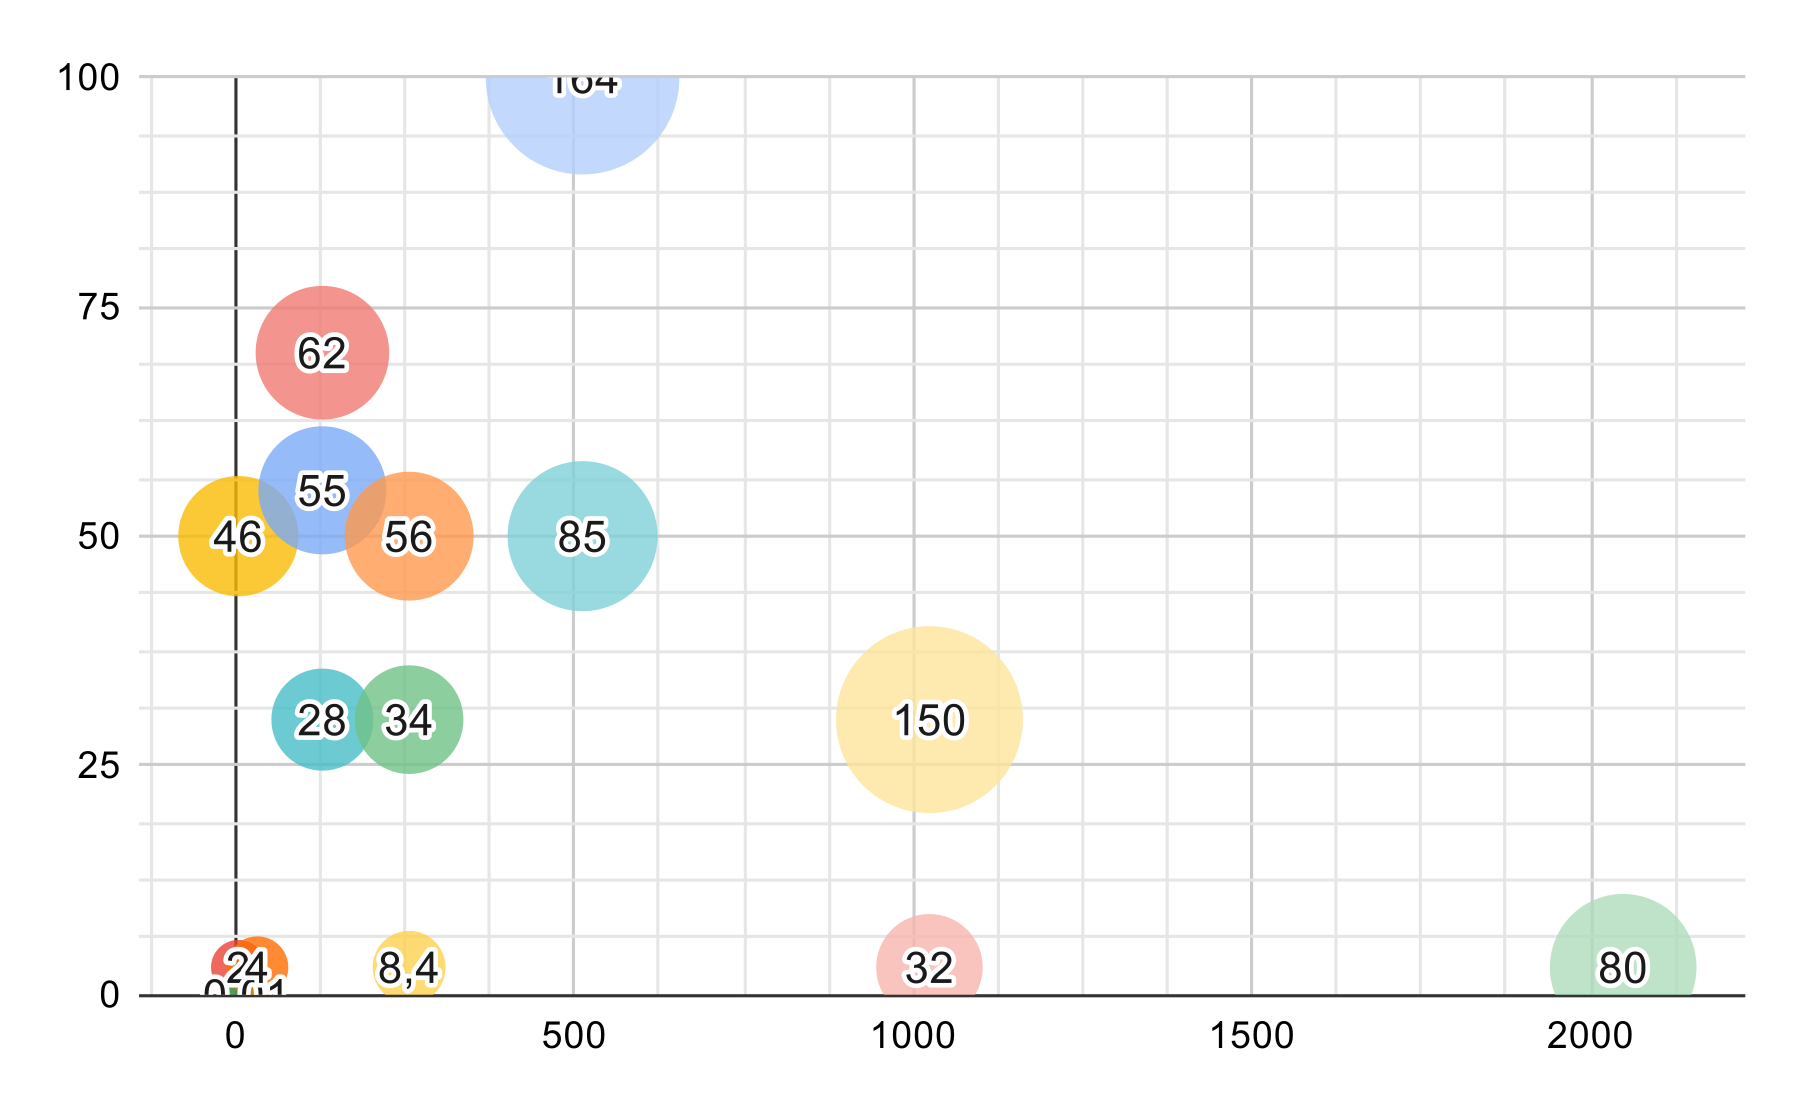
\includegraphics[width=\linewidth]{6_sheets-resources-requirements-compile.png}
		\caption[RAM Compile]{RAM compilation phase. \newline x:users y:transactions}
		\label{fig:7_sheets-resources-requirements-compile.png}
	\end{minipage}%
\end{figure}

\subsection{ZoKrates Rollup Performance\label{subsec:6_zokratesperf}}

A problem that emerges immediately when compiling the ZoKrates programs are the computational requirements to be able to compute the witness and generate a proof to submit to Layer 1. The usage of the Poseidon hash function allowed the compilation of programs using more users and more transactions. Figure \ref{fig:7_sheets-resources-requirements-compile.png} shows the RAM resources needed for the compilation phase of the rollup program\footnote{A GCP machine has been used for RAM usage above 60 GB}. The great complexity increase when adding transactions is due to the fact that the verification of the signature still uses the sha256 hash function. Note that the compilation phase is done only once, and the computation of the witness and generation of the proof are much less demanding, but those results show the complexity growth when adding transactions compared to adding users.

\paragraph{Witness Computation}

Figure \ref{fig:7_sheets-resources-requirements-witness.png} shows the compute-witness phase, which occurs during each rollup computation. This phase executes the ZoKrates program, generating a witness containing the computation results. The witness will then be used to generate a proof of correct computation. The graph demonstrates that the RAM usage during this phase is minimal when compared to the compilation phase. Consequently, ZoKrates programs can effectively run on entry-level machines, and the compilation output file can be shared as it only needs to be computed once. This efficiency in resource utilization brings also the benefit of fast witness computations time for the rollup programs: table \ref{tab:6_witness-proof-time} gives a clear view of the time required to compute the witness. It is evident that an increase in the number of users leads to an almost directly proportional increase in witness computation time within the rollup system. One advantage ZoKrates offers during witness computation is the ability to use all the cores available on the machine, allowing a reduction of witness computation times.

\begin{table}
	\centering
	\begin{tabular}{|c|c|c|c|}
		\hline
		Users & Transactions & witness & proof \\ \hline
		128   & 30           & 1       & 2     \\ \hline
		128   & 55           & 2       & 4     \\ \hline
		128   & 70           & 2       & 5     \\ \hline
		256   & 50           & 2       & 5     \\ \hline
		1024  & 30           & 11      & 20    \\ \hline
	\end{tabular}
	\caption[Witness Proof time]{Witness and proof computation time in minutes.}
	\label{tab:6_witness-proof-time}
\end{table}

\paragraph{Proof Generation}

The proof generation phase is more resource demanding: from Figure \ref{fig:7_sheets-resources-requirements-proof.png} it's clear that the amount of RAM needed is about ten times the RAM used for the witness computation. The benchmarks done for the proof generation phase went up to the maximum of 70 GB for 1024 users and 30 transactions. This is still an affordable amount of RAM for a server, but it's important to highlight that the proof generation phase is the most resource demanding phase of the whole rollup computation. A more plausible scenario for a rollup system would have less transactions and more stale users. This increases the proof phase performance, as less transactions bring the possibility to add large amount of users.

\begin{figure}
	\centering
	\begin{minipage}{.5\textwidth}
		\centering
		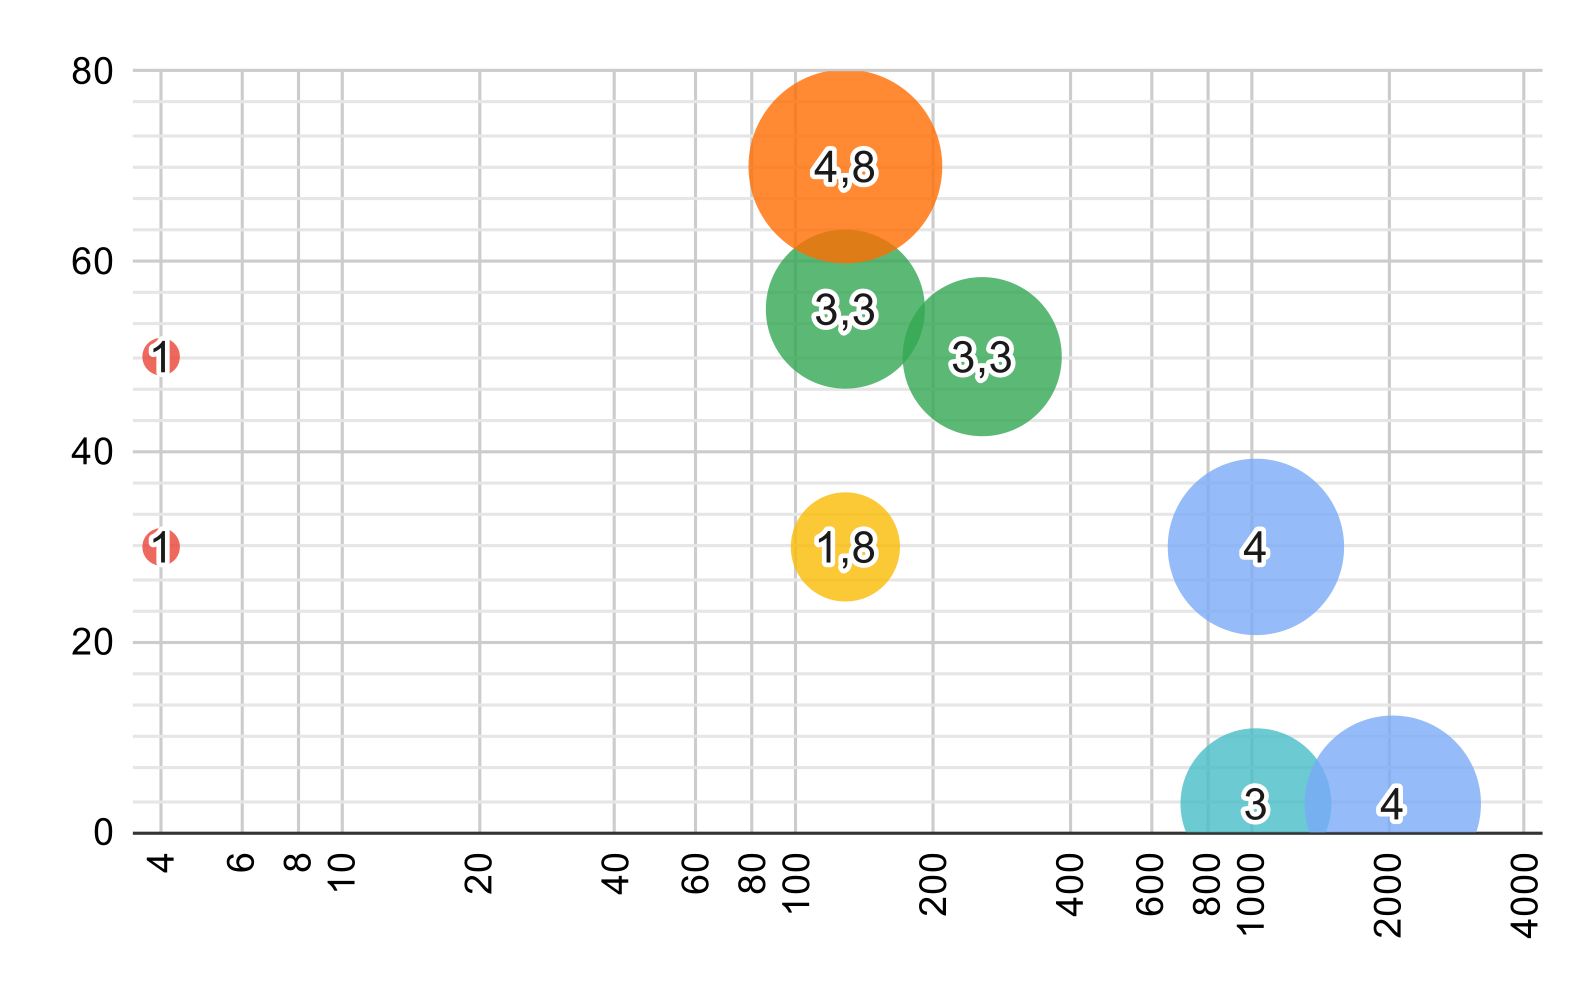
\includegraphics[width=\linewidth]{6_sheets-resources-requirements-witness.png}
		\caption[RAM Compile]{RAM witness phase. \newline x:users y:transactions}
		\label{fig:7_sheets-resources-requirements-witness.png}
	\end{minipage}%
	\begin{minipage}{.5\textwidth}
		\centering
		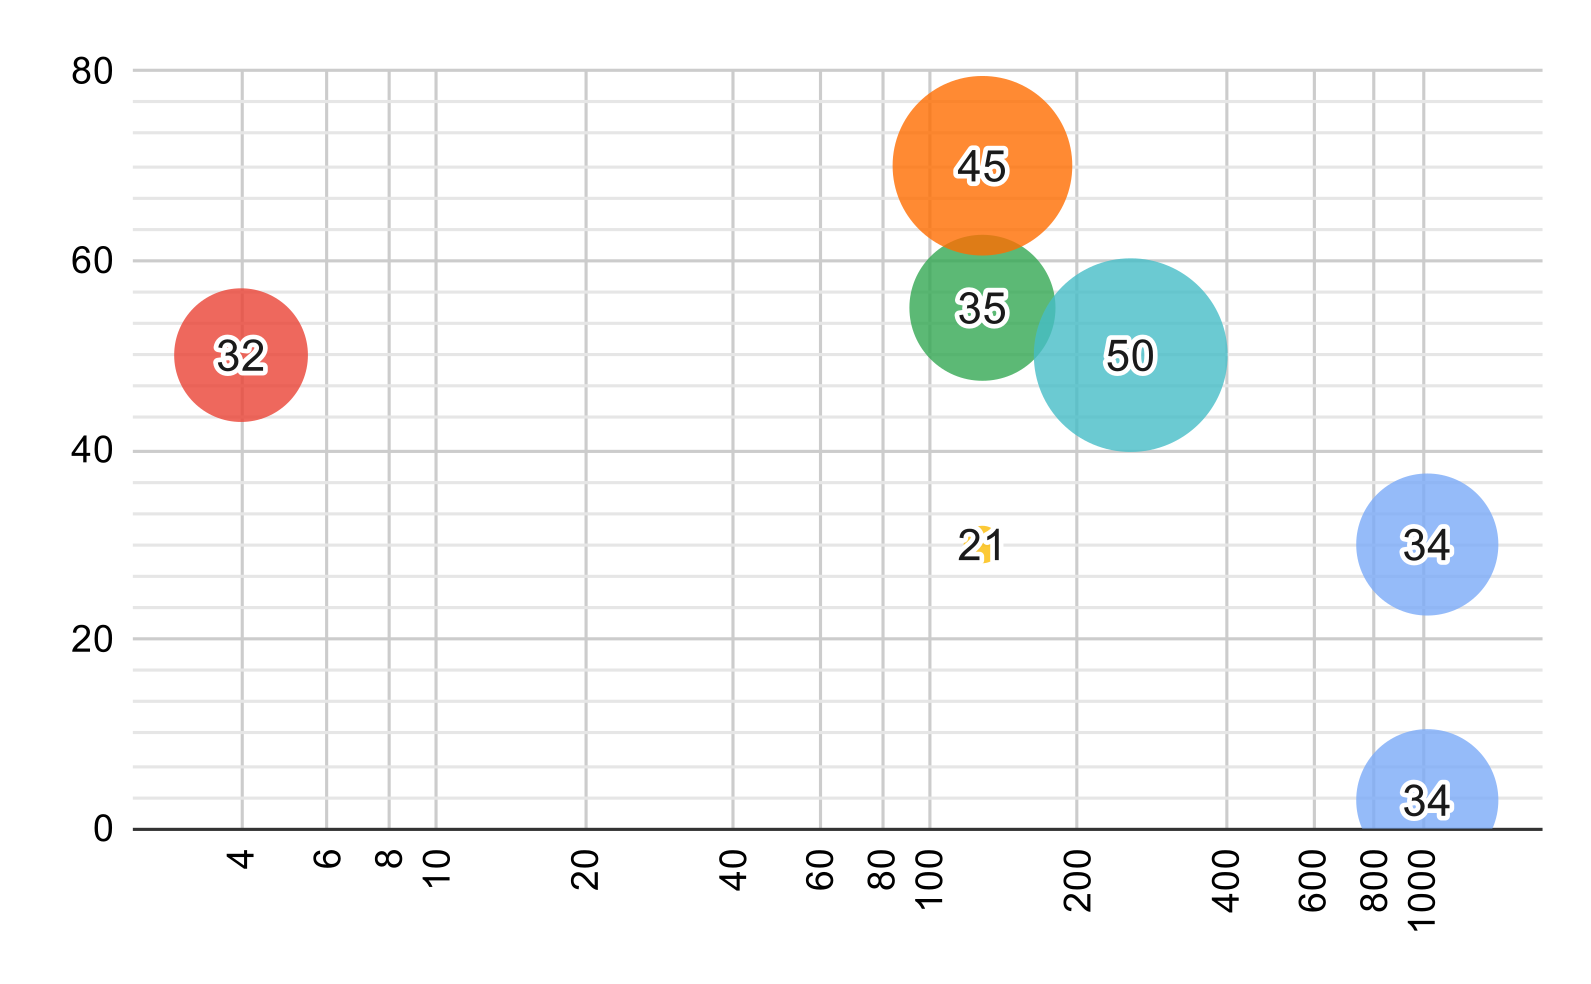
\includegraphics[width=\linewidth]{6_sheets-resources-requirements-proof.png}
		\caption[RAM Proof]{RAM proof phase. \newline x:users y:transactions}
		\label{fig:7_sheets-resources-requirements-proof.png}
	\end{minipage}
\end{figure}

\subsection{Tezos Rollup Fees}

The Tezos Rollup system incurs costs for verification performed by verifier contracts and subsequent storage updates. The verification cost is directly related to the proof's size. During proof verification, each constraint is checked in a loop, consuming gas for each verified constraint. As of 18/08/2023, a single Layer 1 transaction between two users costs 0.000518 tz.

Figure \ref{fig:6_sheets-cost-comparison} presents the fees for a single transaction in various Rollup System size scenarios. These fees are determined by submitting a rollup execution proof and looking at the costs associated with proof verification and storage updates. From the graph it is evident that even with a small Rollup System, fees remain low and always below the fees of a single Layer 1 transaction. While Tezos fees may increase with a higher number of transactions due to the growth in proof size (as explained in Section \ref{sec:5_redandcompr}), the inclusion of more transactions in the rollup system leads to reduced fees overall.

Tezos fees are unaffected by the number of users since the proof contains no user state data, focusing only on the two merkle tree roots and transaction results. This design allows the verifier smart contract to avoid iterating over additional proof fields, which would otherwise consume more gas when more users are involved. Figure \ref{fig:6_sheets-cost-comparison-percentage} presents the percentage of saved fees when using the rollup system in different configurations. This percentage is calculated by comparing the fees of a single Layer 1 transaction with those of a single rollup transaction. The graph demonstrates that as more transactions are included in the rollup system, the fees per transaction decrease, while the addition of users has no impact on costs. When using the rollup system with 1024 users and 30 transactions, fees are reduced by 34\% compared to a single Layer 1 transaction.

\begin{figure}
	\centering
	\begin{minipage}{.5\textwidth}
		\centering
		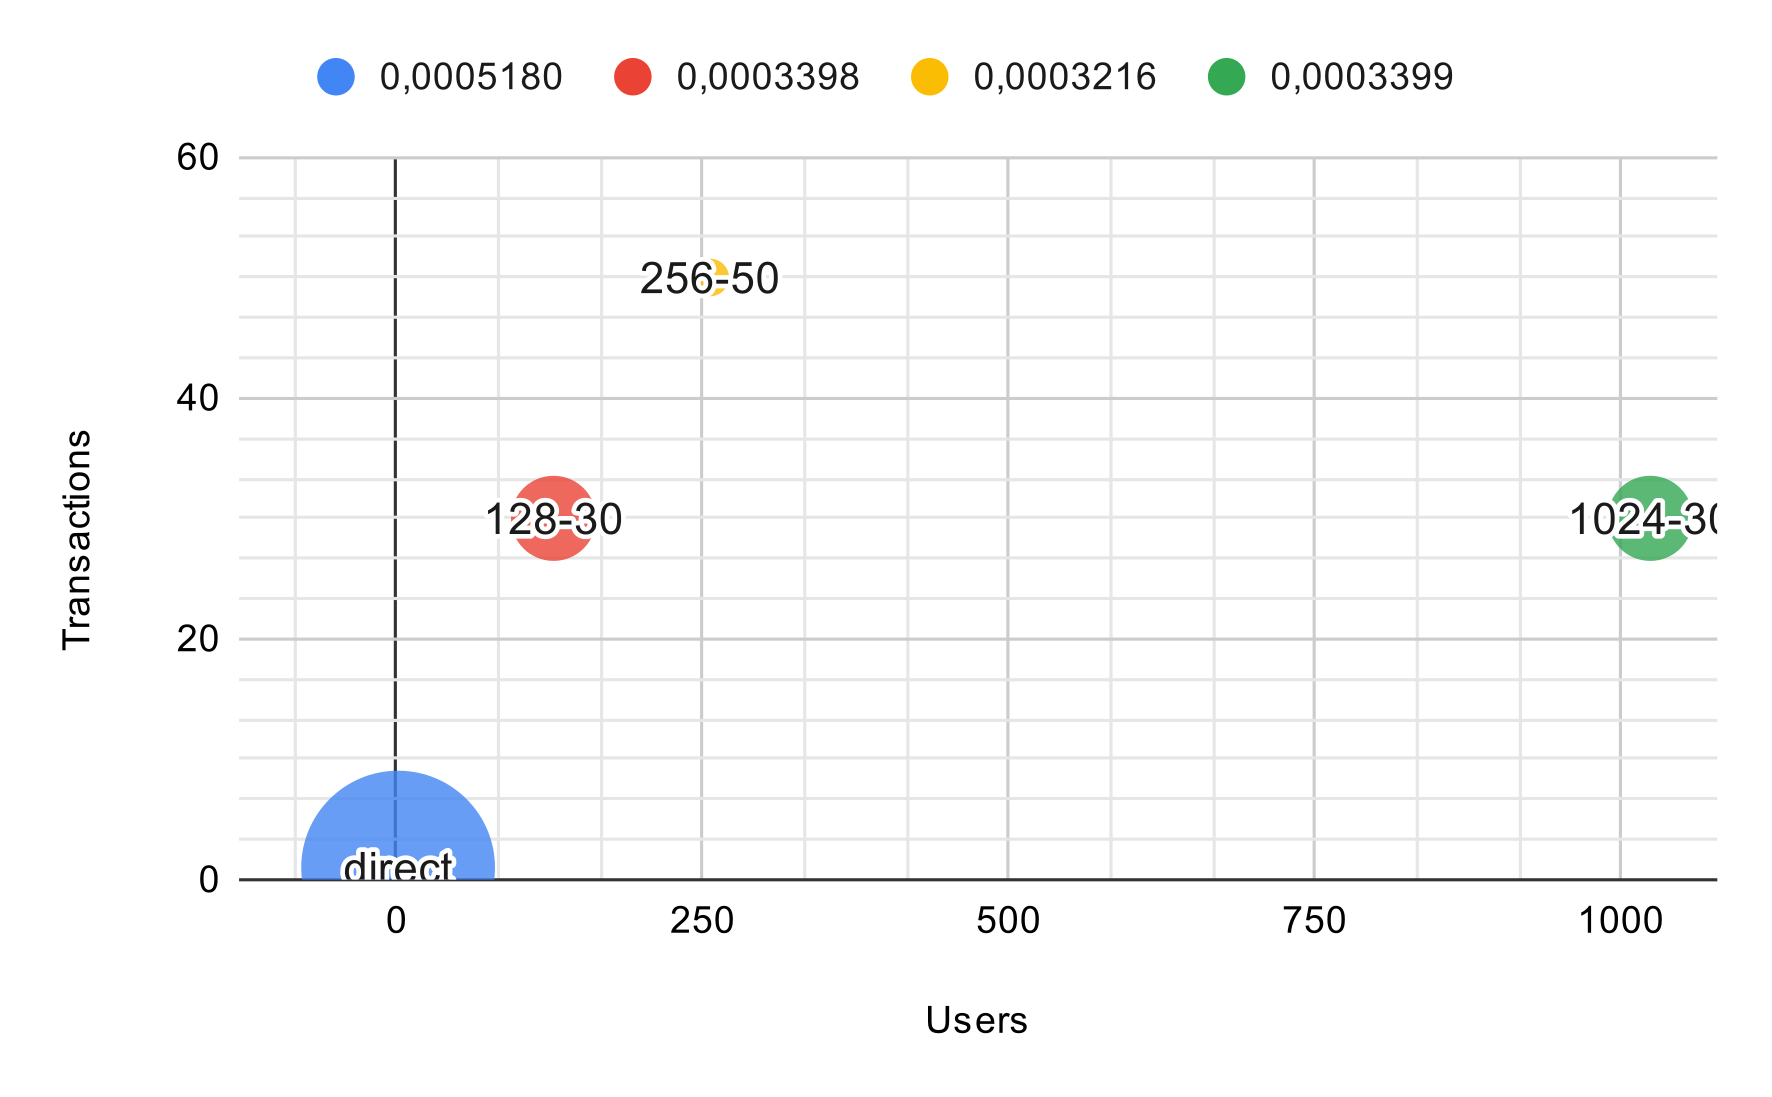
\includegraphics[width=\linewidth]{6_sheets-cost-comparison.png}
		\caption[Cost Comparison]{Cost per Transaction. \newline x:users y:transactions}
		\label{fig:6_sheets-cost-comparison}
	\end{minipage}%
	\begin{minipage}{.5\textwidth}
		\centering
		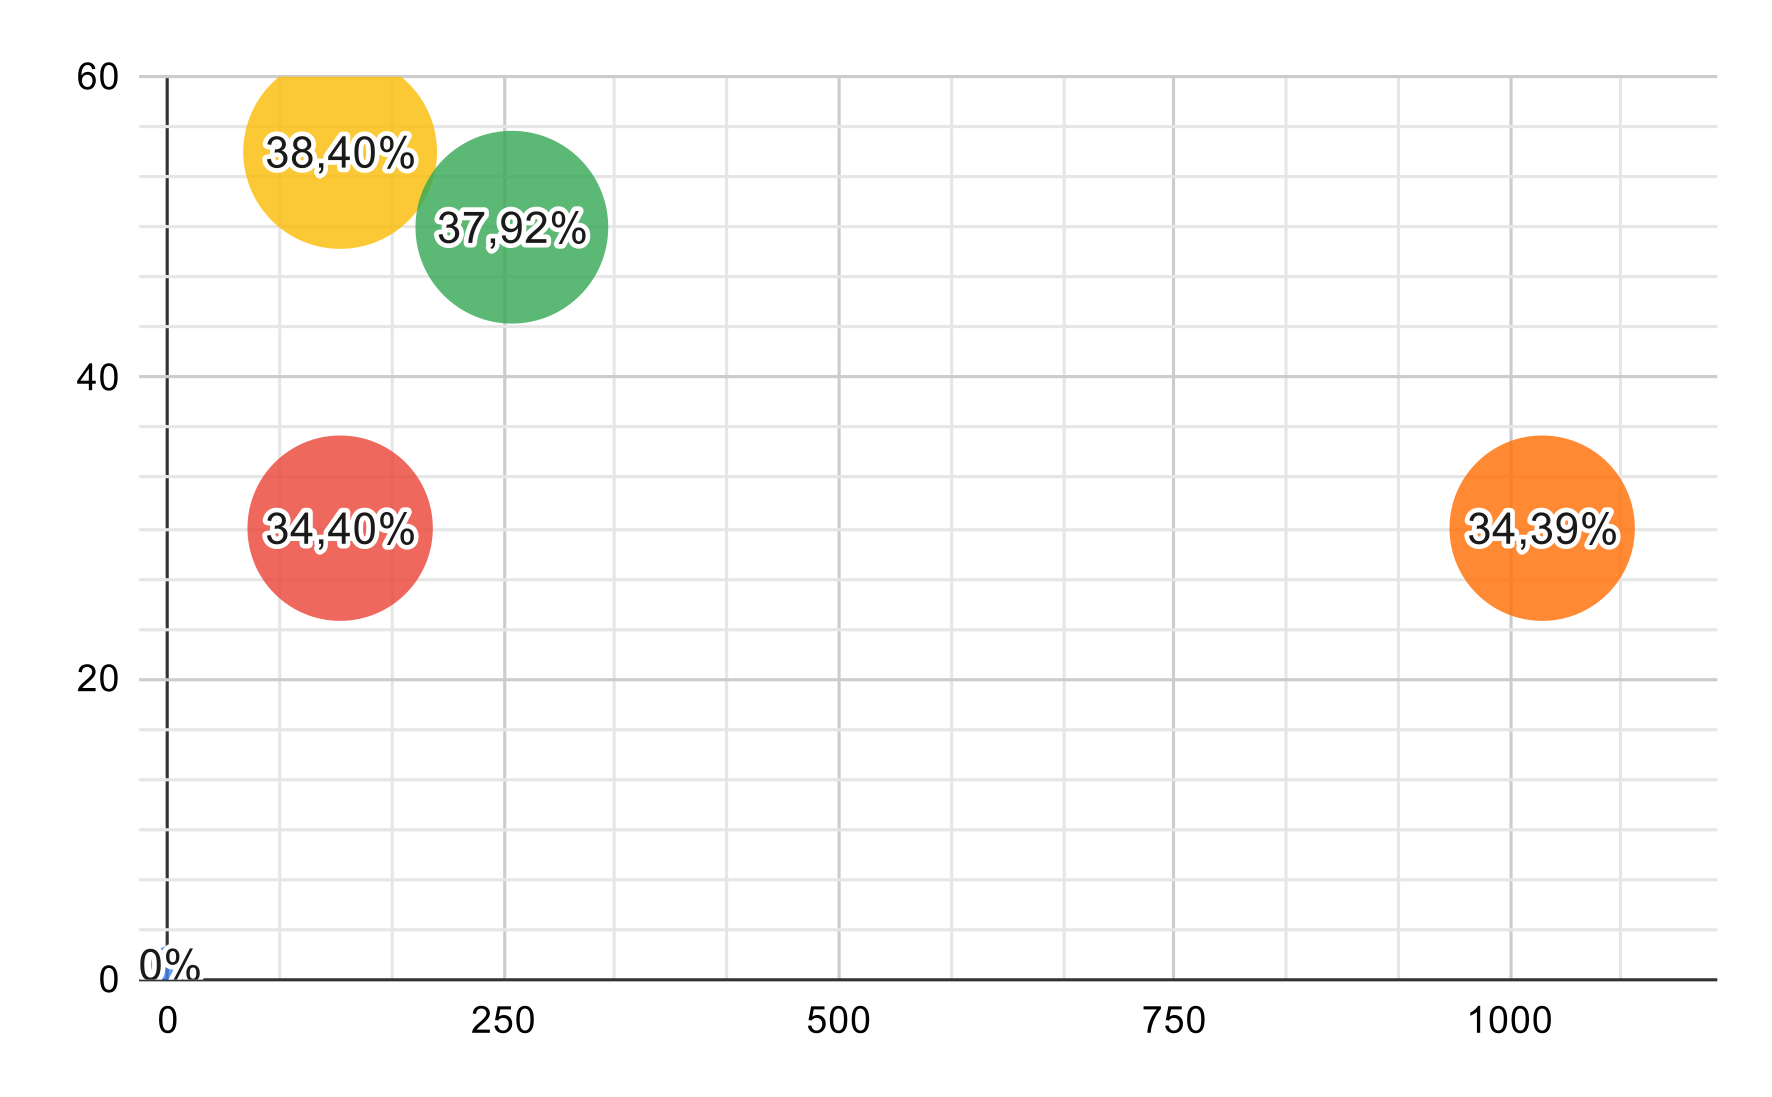
\includegraphics[width=\linewidth]{6_sheets-cost-comparison-percentage.png}
		\caption[Transaction Savings]{Savings per Transaction. \newline x:users y:transactions}
		\label{fig:6_sheets-cost-comparison-percentage}
	\end{minipage}
\end{figure}

\section{Cost Model}

The proposed Rollup System has demonstrated greater efficiency compared to the conventional Layer 1 transaction system. However, there are additional costs that must be considered, including the expenses associated with running Layer 2 servers and the fees required for submitting and verifying proofs. In the current design, these costs are covered by the server submitting the proof. Consequently, the introduction of a fee system for Layer 2 users becomes necessary. It's important to highlight that inactive users on Layer 2 can be problematic, as they inflate the user list, thus increasing the operational costs of the entire rollup system. To address this issue, the implementation of a stale user fee is needed.

\subsection{Stale User Fee\label{subsec:7_staleuserfee}}

In order to execute a rollup, it is necessary to retrieve all users to recalculate the new Merkle root and determine the updated balances. As the number of users registering within the system increases, this process becomes slower. ZoKrates programs are capable of handling only powers of 2 numbers of users (including empty users) due to the merkle tree's structural characteristics. This can lead to exponential growth even when the number of users increases by just one.

Upon registering with the rollup system, a user transfers funds from his account to the Manager Smart Contract. This approach allows the Manager Smart Contract to manage user funds by applying fees under specific circumstances. A proposed Fee Model revolves around the concept of a user's last activity, defined as the most recent event of sending or receiving a transaction within the Rollup System. This information can be easily computed by the Manager Smart Contract while updating balances and nonces for senders and receivers after a successful proof verification: using a Big Map in the storage mapped with the same indexes of the main one it can save the last activity with a timestamp. This Big Map doesn't add overhead to the whole system: it is not included in the rollup programs and only the senders and receivers indexes are accessed (and deserialized) after a successful proof verification.

An external server node may periodically retrieve the Big Map of users activity and identify stale accounts. Through a ZoKrates program that is subsequently verified, the server can compute the updated balances while collecting fees on stale accounts. These fees can then be directly transferred to the Rollup Manager Smart Contract, which can utilize them to cover the costs of proof verification and storage updates.

\subsection{Reward System}

Layer 2 Rollup servers consist of two types: Web-Managers and ZoKrates executors. Web-Managers are economical servers, capable of operating with modest hardware specifications. They function as Docker containers hosting a database and NodeJs server. On the other hand, ZoKrates executors are relatively more resource-intensive, requiring a significant amount of RAM for witness computation and proof generation. However, ZoKrates executors possess an advantage: they don't need to run continuously, being only necessary when computing proofs. This enables them to be deployed on a cloud service and activated only as needed. This approach can reduce the costs of Layer 2 operations.

Similar to the role of bakers in the Tezos blockchain when generating blocks, Layer 2 nodes can be rewarded for their contributions in submitting valid proofs. These rewards are extracted from the sender's balance during a rollup transaction. The rewarded amounts are then accredited directly to the Rollup Manager Smart Contract's Layer 1 balance. This enables the Rollup Manager Smart Contract to pay a baker for the proof submission without requiring an update of the Merkle Tree of the balances, because its balance is a direct amount stored in L1.

\section{Scalability}

Achieving scalability when using zero knowledge proofs is a challenge due to the high amount of resources needed to run the computational phase of zk programs. The time needed to finalize the proof generation is also a factor that limits the scalability of the system. Considering table \ref{tab:6_witness-proof-time} it takes a total of 31 minutes, using the test machine, to generate a valid proof for 30 transactions to be submitted to the Rollup-Manager contract. This is a slower result than having the transactions executed directly on the main chain. Taking an ideal blockchain use where all the applications use a Rollup System, it would mean that, in the rollup configuration of 30 transactions, the total amount of interaction with Layer 1 would be reduced by $1/30$, having ideally 30 times the transaction throughput. This value can easily be increased by increasing the computing power of the machine running the ZoKrates program, as the witness and proof generation take advantage of all the cores available on the machine.

\subsection{Scalability Improvements}

The proposed Rollup System is capable of running in a ideal environment, where there are no spikes of demand and only one server running. If more servers would run a major problem would arise. When the ZoKrates program begins the witness computation it gets as input a state of the rollup system represented by the two merkle roots and by the user Big Map. If a L2 rollup system starts the rollup computation with a set of transactions \textit{A} and submitting a valid proof while another L2 rollup system is still computing another transaction set \textit{B}, the proof of the set \textit{B} will be rejected even if the transactions were applied correctly and they were influencing different users by the set \textit{A}. This is due to the fact that the Manager Smart Contract checks for the input roots of the ZoKrates program to match the roots in its storage, to prove that the initial state was the same and was not altered. This problem has not been solved in this prototype yet.

Here's an initial proposal: the user list can be split in two or more parts, each one having its own merkle root, one for the users public keys and the other for the balances and nonces. Let's pretend we split the users in three groups. The most efficient scenario is that all the transactions received by a node involve users from the same group: this would allow the rollup system to run in parallel on three different servers, each one executing ZoKrates program and sending proofs that will interfere with each other. In a real case scenario there will be transactions involving users from different groups, and this will require the rollup system to run on a single server, as the ZoKrates program will change more than one balance and nonce merkle tree. A proposed solution is to have redirected all the transactions within the same group to a single server that manages this particular group, while the transactions with mixed users in another; this decreases the chances of having to recompute the rollup with the newer state fetched from the Manager Smart Contract. This solution is not ideal, as it requires a more complex management of the rollup system, but it's a starting point to improve the scalability of the system.